\documentclass[tikz,border=5pt]{standalone}
\usepackage{amsmath}
\usetikzlibrary{arrows.meta,calc}
\tikzset{rayi/.style={blue!65!black,thick,-{Stealth[length=2mm]}},
rayt/.style={red!70!black,thick,-{Stealth[length=2mm]}},
guide/.style={gray!65,dashed,thin},
axis/.style={black!65,thin,-{Stealth[length=2mm]}},
dim/.style={thin}}
\begin{document}
% statement-07: exact physical branch X=-(2+sqrt(1+3Y^2))/3, f=1.
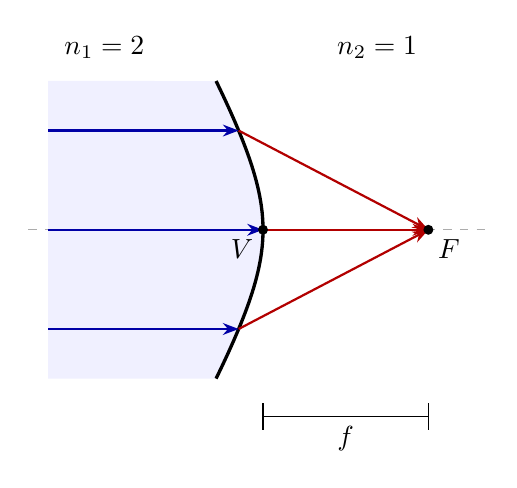
\begin{tikzpicture}[x=2.1cm,y=2.1cm]
\fill[blue!6] (-2.3,-.9)--plot[domain=-.9:.9,samples=60] ({-(2+sqrt(1+3*\x*\x))/3},\x)--(-2.3,.9)--cycle;
\draw[guide] (-2.42,0)--(.36,0);
\draw[very thick] plot[domain=-.9:.9,samples=60] ({-(2+sqrt(1+3*\x*\x))/3},\x);
\foreach \h in {-.6,0,.6}{
 \pgfmathsetmacro{\surfX}{-(2+sqrt(1+3*\h*\h))/3}
 \draw[rayi] (-2.3,\h)--(\surfX,\h);
 \draw[rayt] (\surfX,\h)--(0,0);}
\fill (0,0) circle[radius=1.8pt] (-1,0) circle[radius=1.8pt];
\node[below right] at (0,0) {$F$};\node[below left] at (-1,0) {$V$};
\node at (-1.96,1.10) {$n_1=2$};\node at (-.31,1.10) {$n_2=1$};
\draw[dim] (-1,-1.13)--(0,-1.13);
\draw[dim] (-1,-1.05)--(-1,-1.21) (0,-1.05)--(0,-1.21);
\node[below] at (-.5,-1.13) {$f$};
\end{tikzpicture}

% optical-07: common plane Xa=-2.15; P at height .8, actual X=-1.236267.
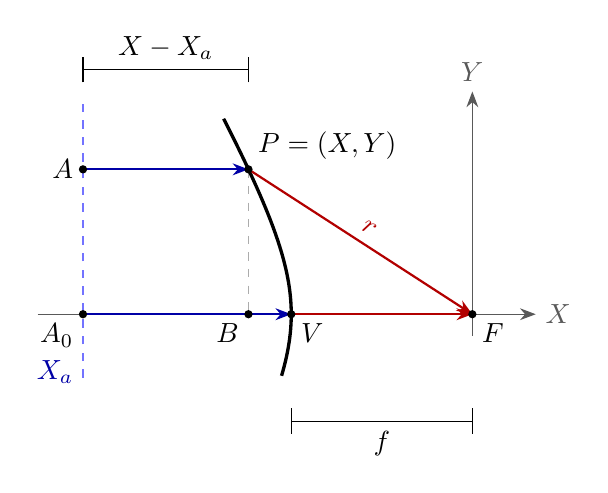
\begin{tikzpicture}[x=2.3cm,y=2.3cm]
\pgfmathsetmacro{\surfX}{-(2+sqrt(1+3*.8*.8))/3}
\coordinate (A) at (-2.15,.8);\coordinate (A0) at (-2.15,0);
\coordinate (P) at (\surfX,.8);\coordinate (B) at (\surfX,0);
\coordinate (V) at (-1,0);\coordinate (F) at (0,0);
\draw[guide,blue!55] (-2.15,-.35)--(-2.15,1.17);
\draw[guide] (P)--(B);
\draw[axis] (-2.4,0)--(.35,0) node[right] {$X$};
\draw[axis] (0,-.12)--(0,1.23) node[above] {$Y$};
\draw[very thick] plot[domain=-.34:1.08,samples=70] ({-(2+sqrt(1+3*\x*\x))/3},\x);
\draw[rayi] (A)--(P);\draw[rayt] (P)--(F) node[midway,above,sloped] {$r$};
\draw[rayi] (A0)--(V);\draw[rayt] (V)--(F);
\foreach \p in {A,A0,P,B,V,F}{\fill (\p) circle[radius=1.5pt];}
\node[left] at (A) {$A$};\node[below left] at (A0) {$A_0$};
\node[above right] at (P) {$P=(X,Y)$};
\node[below left] at (B) {$B$};\node[below right] at (V) {$V$};
\node[below right] at (F) {$F$};
\draw[dim] (-2.15,1.35)--(\surfX,1.35);
\draw[dim] (-2.15,1.28)--(-2.15,1.42) (\surfX,1.28)--(\surfX,1.42);
\node[above] at ({(-2.15+\surfX)/2},1.35) {$X-X_a$};
\draw[dim] (-1,-.59)--(0,-.59);
\draw[dim] (-1,-.52)--(-1,-.66) (0,-.52)--(0,-.66);
\node[below] at (-.5,-.59) {$f$};
\node[blue!65!black,left] at (-2.15,-.32) {$X_a$};
\end{tikzpicture}

% snell-07: exact normal and actual transmitted direction at Y=.8f.
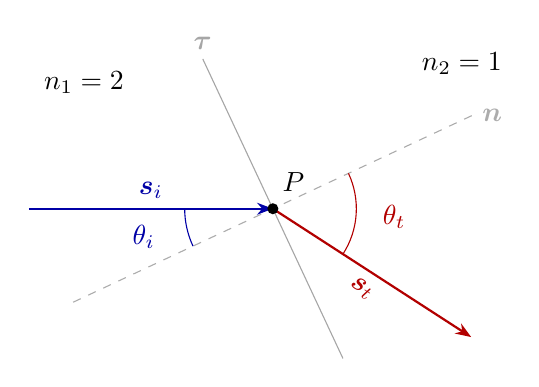
\begin{tikzpicture}[x=2cm,y=2cm]
\pgfmathsetmacro{\surfX}{-(2+sqrt(1+3*.8*.8))/3}
\pgfmathsetmacro{\rayR}{-1-2*\surfX}
\pgfmathsetmacro{\dX}{-\surfX/\rayR}\pgfmathsetmacro{\dY}{-.8/\rayR}
\pgfmathsetmacro{\slope}{-.8/sqrt(1+3*.8*.8)}
\pgfmathsetmacro{\normLen}{sqrt(1+\slope*\slope)}
\pgfmathsetmacro{\nX}{1/\normLen}\pgfmathsetmacro{\nY}{-\slope/\normLen}
\pgfmathsetmacro{\tX}{\slope/\normLen}\pgfmathsetmacro{\tY}{1/\normLen}
\pgfmathsetmacro{\angleN}{atan(-\slope)}\pgfmathsetmacro{\angleT}{atan(\dY/\dX)}
\draw[gray!70] ({-1.05*\tX},{-1.05*\tY})--({1.05*\tX},{1.05*\tY}) node[above] {$\boldsymbol\tau$};
\draw[guide] ({-1.4*\nX},{-1.4*\nY})--({1.4*\nX},{1.4*\nY}) node[right] {$\boldsymbol n$};
\draw[rayi] (-1.55,0)--(0,0) node[midway,above] {$\boldsymbol s_i$};
\draw[rayt] (0,0)--({1.5*\dX},{1.5*\dY}) node[midway,below,sloped] {$\boldsymbol s_t$};
\draw[blue!65!black] (180:.56) arc[start angle=180,end angle={180+\angleN},radius=.56];
\node[blue!65!black] at (-.82,-.18) {$\theta_i$};
\draw[red!70!black] (\angleT:.53) arc[start angle=\angleT,end angle=\angleN,radius=.53];
\node[red!70!black] at (.77,-.05) {$\theta_t$};
\fill (0,0) circle[radius=2pt];\node[above right] at (0,.05) {$P$};
\node at (-1.2,.8) {$n_1=2$};\node at (1.2,.92) {$n_2=1$};
\end{tikzpicture}

% spatial-07: genuinely curved meridians; Y,Z projection basis (0,1),(.62,.30).
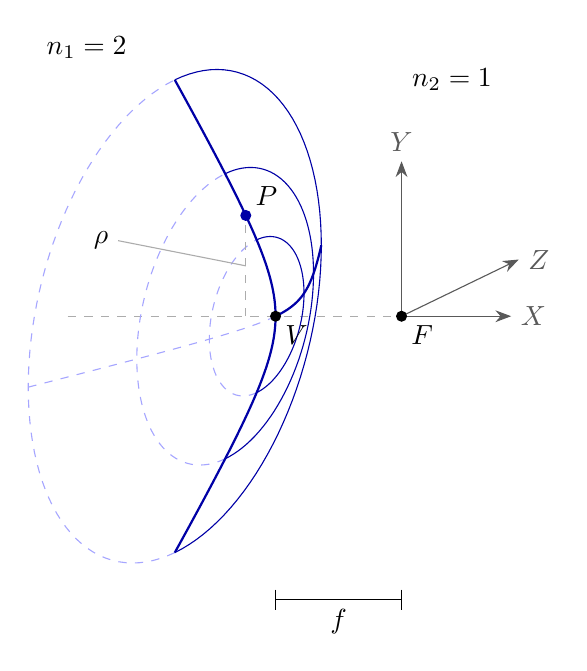
\begin{tikzpicture}[x=1.6cm,y=1.6cm]
\draw[guide] (-2.65,0)--(0,0);
\foreach \longX in {-1.8,-1.4,-1.15}{
 \pgfmathsetmacro{\radiusR}{sqrt(3*\longX*\longX+4*\longX+1)}
 \draw[blue!35,dashed] plot[domain=180:360,samples=65] ({\longX+.62*\radiusR*sin(\x)},{\radiusR*cos(\x)+.30*\radiusR*sin(\x)});
 \draw[blue!65!black] plot[domain=0:180,samples=65] ({\longX+.62*\radiusR*sin(\x)},{\radiusR*cos(\x)+.30*\radiusR*sin(\x)});}
\foreach \ang in {0,90,180}{
 \draw[blue!65!black,thick] plot[domain=0:1.876166,samples=65] ({-(2+sqrt(1+3*\x*\x))/3+.62*\x*sin(\ang)},{\x*cos(\ang)+.30*\x*sin(\ang)});}
\draw[blue!35,dashed] plot[domain=0:1.876166,samples=65] ({-(2+sqrt(1+3*\x*\x))/3-.62*\x},{-.30*\x});
\draw[axis] (0,0)--(.87,0) node[right] {$X$};
\draw[axis] (0,0)--(0,1.23) node[above] {$Y$};
\draw[axis] (0,0)--(.93,.45) node[right] {$Z$};
\pgfmathsetmacro{\surfX}{-(2+sqrt(1+3*.8*.8))/3}
\draw[guide] (\surfX,0)--(\surfX,.8);
\draw[gray!65,thin] (-2.25,.60)--(\surfX,.40);
\node[left] at (-2.25,.60) {$\rho$};
\fill[blue!65!black] (\surfX,.8) circle[radius=2pt];\node[above right] at (\surfX,.8) {$P$};
\fill (-1,0) circle[radius=2pt] (0,0) circle[radius=2pt];
\node[below right] at (-1,0) {$V$};\node[below right] at (0,0) {$F$};
\draw[dim] (-1,-2.25)--(0,-2.25);
\draw[dim] (-1,-2.17)--(-1,-2.33) (0,-2.17)--(0,-2.33);
\node[below] at (-.5,-2.25) {$f$};
\node at (-2.5,2.13) {$n_1=2$};\node at (.4,1.88) {$n_2=1$};
\end{tikzpicture}

% moving-07: rest and ground t=0 slices, identical transverse scale; longitudinal factor .6.
\begin{tikzpicture}[x=1.8cm,y=1.8cm]
\begin{scope}
\node at (-.67,1.26) {$S'$};
\draw[guide] (-1.75,0)--(.27,0);
\draw[very thick,blue!65!black] plot[domain=-.85:.85,samples=65] ({-(2+sqrt(1+3*\x*\x))/3},\x);
\fill (-1,0) circle[radius=1.8pt] (0,0) circle[radius=1.8pt];
\node[below left] at (-1,0) {$V$};\node[below right] at (0,0) {$F$};
\draw[dim] (-1,-1.02)--(0,-1.02);
\draw[dim] (-1,-.94)--(-1,-1.1) (0,-.94)--(0,-1.1);
\node[below] at (-.5,-1.02) {$f$};
\end{scope}
\begin{scope}[xshift=5.4cm]
\node at (-.52,1.26) {$S,\quad t=0$};
\draw[guide] (-1.35,0)--(.7,0);
\draw[very thick,red!70!black] plot[domain=-.85:.85,samples=65] ({-.6*(2+sqrt(1+3*\x*\x))/3},\x);
\fill (-.6,0) circle[radius=1.8pt] (0,0) circle[radius=1.8pt];
\node[below left] at (-.6,0) {$V_t$};\node[below right] at (0,0) {$F_t$};
\draw[dim] (-.6,-1.02)--(0,-1.02);
\draw[dim] (-.6,-.94)--(-.6,-1.1) (0,-.94)--(0,-1.1);
\node[below] at (-.3,-1.02) {$3f/5$};
\draw[axis,red!70!black,thick] (.03,.31)--(.67,.31) node[midway,above] {$v$};
\end{scope}
\end{tikzpicture}

% events-07: longitudinal projection only, not a 1+1-dimensional null diagram for oblique ray.
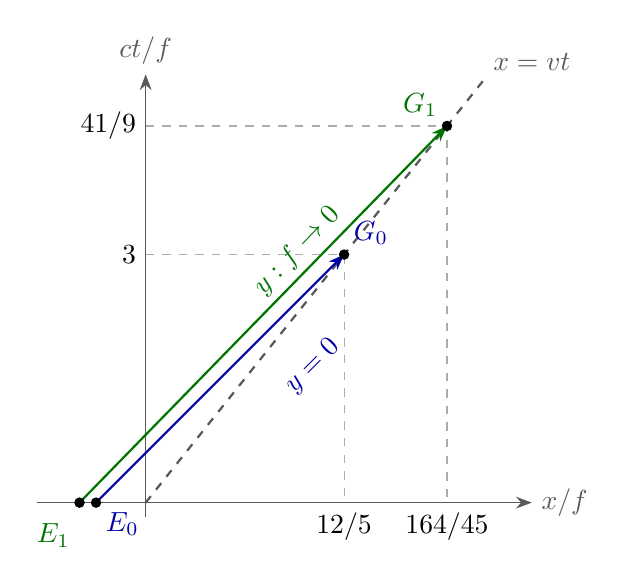
\begin{tikzpicture}[x=1.05cm,y=1.05cm]
\draw[axis] (-1.32,0)--(4.67,0) node[right] {$x/f$};
\draw[axis] (0,-.18)--(0,5.18) node[above] {$ct/f$};
\draw[guide,black!65,thick] (0,0)--(4.08,5.1) node[above right] {$x=vt$};
\draw[rayi] (-.6,0)--(2.4,3);
\draw[green!45!black,thick,-{Stealth[length=2mm]}] (-.8,0)--({164/45},{41/9});
\draw[guide] (0,3)--(2.4,3)--(2.4,0);
\draw[guide] (0,{41/9})--({164/45},{41/9})--({164/45},0);
\foreach \xx/\yy in {-.6/0,-.8/0,2.4/3,{164/45}/{41/9}}{\fill (\xx,\yy) circle[radius=1.9pt];}
\node[blue!65!black,below right] at (-.6,0) {$E_0$};
\node[green!45!black,below left] at (-.8,-.14) {$E_1$};
\node[blue!65!black,above right] at (2.4,3) {$G_0$};
\node[green!45!black,above left] at ({164/45},{41/9}) {$G_1$};
\node[left] at (0,3) {$3$};\node[left] at (0,{41/9}) {$41/9$};
\node[below] at (2.4,0) {$12/5$};\node[below] at ({164/45},0) {$164/45$};
\node[blue!65!black,rotate=45] at (2.02,1.65) {$y=0$};
\node[green!45!black,rotate=46] at (1.83,3.05) {$y:f\to0$};
\end{tikzpicture}
\end{document}
